%%%%%%%%%%%%%%%%%%%%%%%%%%%%%%%%%%%%%%%%%%%%%%%%%%%%%%%%%%%%%%%%%%%%%%%%%%%%%%%%%%%%%%%%%%%
%                               My System 24pp
%%%%%%%%%%%%%%%%%%%%%%%%%%%%%%%%%%%%%%%%%%%%%%%%%%%%%%%%%%%%%%%%%%%%%%%%%%%%%%%%%%%%%%%%%%%
\chapter{Architecture}
\label{sec:Architecture}
 
%%%%%%%%%%%%%%%%%%%%%
 
\section*{Summary}

In this chapter we will present the details we propose regarding Floodgate's architecture. In first place, on Sect. \ref{sec:floodgate-overview}, we will present a brief overview of our system. Then, in Sect. \ref{sec:building-blocks}, we will present and justify the building blocks in which our mobile-server architecture is based, talking about the IFC models implemented on each end. After that, we will present the programming and deployment model which developers must follow in order to produce Floodgate-ready applications, on Sect. \ref{sec:programming-model}. Then, we will provide a detailed explanation of how we achieve the end-to-end taint tracking and how we deal with taint persistence on the server-side, on Sect. \ref{sec:end-to-end-taint-tracking} and \ref{sec:server-side-taint-persistence}, respectively.

In the next chapter we present the implementation details for the proposed architecture.

\section{Floodgate Overview}
\label{sec:floodgate-overview}

We propose Floodgate, a system that will rely on a mobile-server architecture to ensure the end-to-end enforcement of specified security policies (SP) across the whole system, as represented on Fig. \ref{fig:floodgate-arch}. Compared to the existing systems, Floodgate will work at \textit{middleware-level}, enforcing security policies in an end-to-end way between mobile-side applications and server-side \textit{backend} supporting those applications. In Floodgate, security policies are specified by the service provider and accepted by the user upon the installation of a mobile application supported by our system (1). On one side, the mobile device running the Android operating system performs an application-level tracking of sensitive data across third-party applications, adding policy checks that prevent the undesired exportation of private data, accordingly with specified security policies. By application-level tracking we mean that, in Floodgate, we follow a more coarse-grained tainting approach, applying taints to the whole application instead of data variables present in the application's data flow. When the application is marked as tainted and data is sent to remote \textit{endpoints} (2) through the taint sinks (e.g. network interfaces), this data has to keep the application's taint marks and security policies assigned, in order to achieve the enforcement of those policies on the application server-side. The server-side operates inside a secure container that is responsible for the policies' enforcement and which provides data declassification mechanisms for secure content sharing between applications running in the same container (3) and support for third-party applications interaction (4).

\begin{figure}[t!]
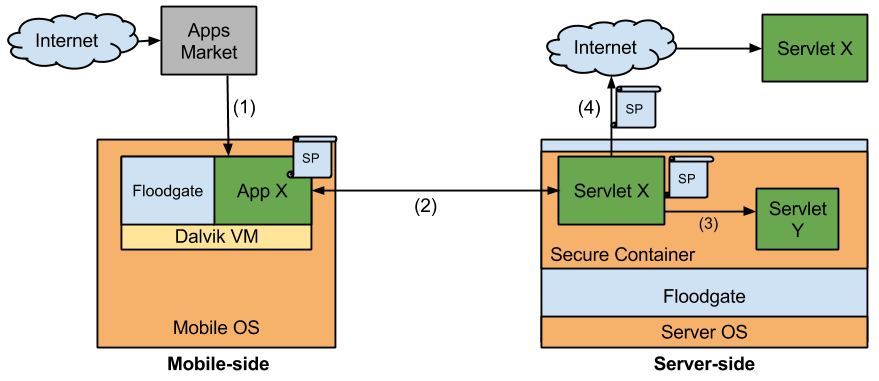
\includegraphics[width=\textwidth]{figs/floodgate-arch}
\centering
\caption{Floodgate proposed architecture}
\label{fig:floodgate-arch}
\end{figure}

\section{Building Blocks}
\label{sec:building-blocks}

As stated in Sect. \ref{sec:floodgate-overview}, Floodgate relies on a mobile-server architecture with components operating on each side. Due to that, we can spot two distinct building blocks, which we now detail.

\subsection{Mobile-side Blocks}
\label{sec:mobile-side-blocks}

On the \textbf{mobile-side}, Floodgate extends common mobile applications with two components, in order to achieve the application-level taint tracking: A text file \textbf{permissions manifest} that is produced by the developer and included in the application's resources; and a library archive, to be specified as a target application's dependency. Both components and the way they interact with the mobile application are represented in Fig. \ref{fig:floodgate-mobile-blocks}.

\begin{figure}[t!]
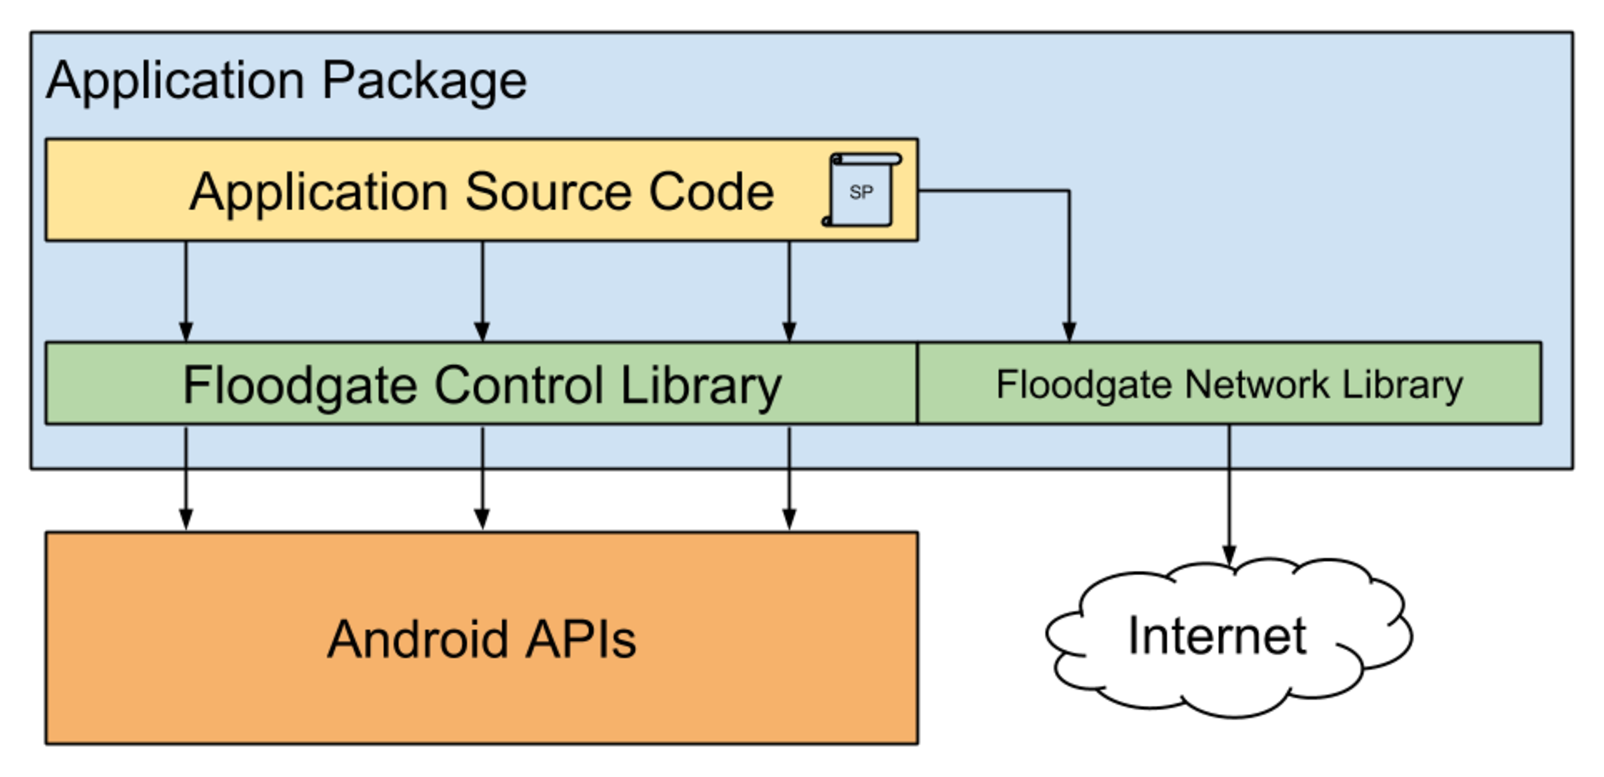
\includegraphics[width=0.6\textwidth]{figs/floodgate-mobile-blocks}
\centering
\caption{Floodgate mobile component design}
\label{fig:floodgate-mobile-blocks}
\end{figure}

The permissions manifest (SP in Figs. \ref{fig:floodgate-arch} and \ref{fig:floodgate-mobile-blocks}) is a data structure which specifies multiple sensitive mobile resources (the device's IMEI, GPS/GSM location, phone number, etc.) along with a key defining the privacy of each resource (public/private). Also, it specifies a list of trusted network \textit{endpoints} with whom the application is allowed to share private resources with. In Floodgate, a public resource is allowed to be sent through the network to any \textit{endpoint}, while a private resource can only be sent to \textit{endpoints} listed as trusted.

The Floodgate's library, by its turn, is comprised by two modules: The control library, which contains the behavior of controlling the access to the resources specified in the permissions manifest and their propagation, and network library, which enables communication over the network. Since Floodgate actually performs an application-level taint tracking on the mobile-side, this library initializes a data structure containing the application taint. This taint is updated when accesses to sensitive resources, specified in the permissions manifest, are detected. In order to detect when the sensitive resources are accessed, the library relies on aspect-oriented programming (AOP) concepts.

AOP relies on partitioning program logic into multiple ``concerns'' (cohesive areas of functionality). With AOP, it's possible to define source code blocks (``cross-cutting concerns'') to be executed before/after/instead another piece of code without explicitly changing it. This way, the ``cross-cutting concerns'' can be implemented once and injected wherever it is needed. The combination of the particular point in a program that might be the target of code injection and the code to be injected is called an \textit{aspect}. Then, the process of injecting code is called \textit{weaving}.

Our library features multiple concerns to be injected when the execution of methods that access a sensitive resource is detected. On such situations, the application taint is updated, always reflecting the resources accessed by the application's source code.

Apart from that, our mobile library also provides methods to communicate with remote \textit{endpoints} over the network.
\todo{Write the network methods available? (in an abstract way, like post(String, Endpoint), get(Endpoint),...)}
These methods ensure that the application taint is always sent along with data, in a transparent way for the developers. In order to enforce this taint propagation through the network, the library features some ``concerns'' regarding the access to other network libraries instead of ours, blocking its execution.

\subsection{Server-side Blocks}
\label{sec:server-side-blocks}

On the \textbf{server-side}, Floodgate provides a secure container where to deploy the \textit{backend} of mobile applications. As referred in Sect. \ref{sec:mobile-side-blocks}, the Floodgate network library deals with the propagation of application taints to the server-side. 

In order to continue the enforcement of such security policies on the server-side, we apply concepts of static analysis, instrumentation and dynamic taint tracking. Every \textit{servlet} running on the Floodgate's secure container has to pass through an \textit{a priori} process of static analysis, graphically presented on Fig. \ref{fig:floodgate-server-blocks}. This process consists in identifying the points in the application where tainted data enters the system, named taint sources (e.g. interfaces to receive network requests coming from the respective mobile application), where it is passed (e.g. variables assignment, methods return) and where it may leave the system (e.g. output network interfaces, database connectors), which we refer to as taint sinks. After the analysis process, Floodgate instruments the application, applying code injection in order to propagate taints wherever the static analysis process dictates to. Finally, we apply dynamic taint tracking in order to keep track of when tainted data are set to leave the system, acting accordingly. Also, Floodgate features a taint persistence module, ensuring that taints entering the \textit{backend} are persistently stored along with data they refer to, avoiding taint loss due to in-memory storage only.

\begin{figure}[t!]
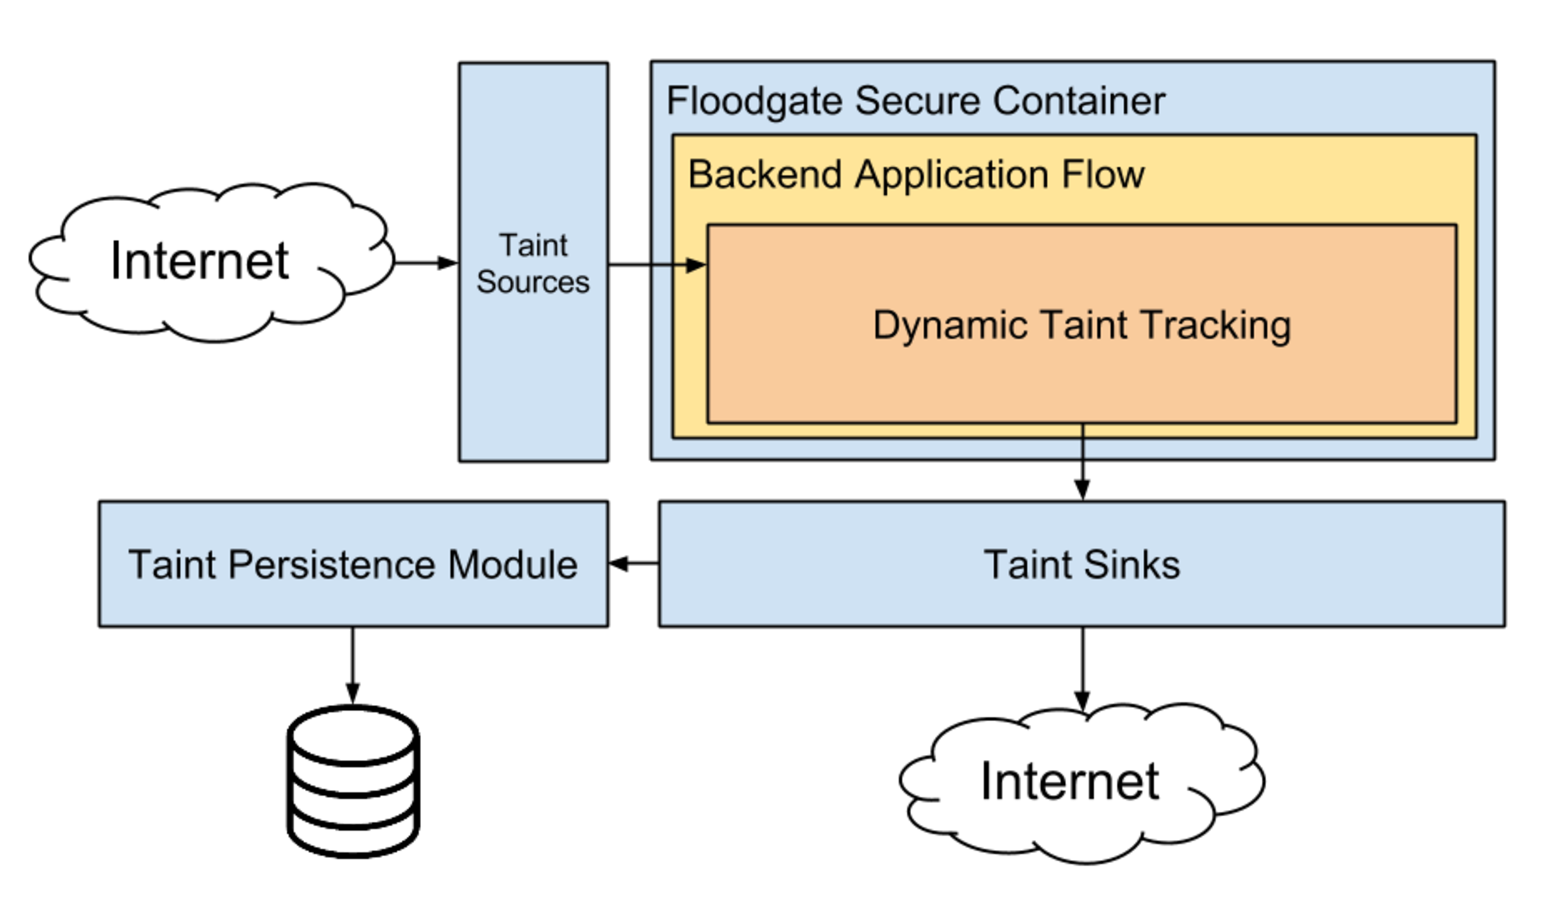
\includegraphics[width=0.6\textwidth]{figs/floodgate-server-blocks}
\centering
\caption{Floodgate server component design}
\label{fig:floodgate-server-blocks}
\end{figure}

\todo{Review the above paragraph. And also, anything more to add? Seems a bit short. The figure also doesn't convince me.}

\section{Programming Model}
\label{sec:programming-model}

Floodgate offers a programming and deployment model specifically targeted to \textit{backend}-supported mobile applications. 

On the \textbf{mobile-side}, the programming model doesn't suffer any major modifications, since developers only need to add the Floodgate mobile library as a dependency for the mobile application and the permissions manifest as an application's resource. After that, developers don't need to worry about anything else regarding data protection and just have to follow normal development process. The only reservation is that developers must use the network methods offered by Floodgate's mobile library to communicate with remote \textit{endpoints}, since they are a key part on the end-to-end taint tracking process. Also, the deployment process for a Floodgate mobile application doesn't suffer any modifications when comparing to the current model.

On the \textbf{server-side}, Floodgate's programming model is essentially based on the definition of a REST API to be deployed on the secure container. This API must offers methods representing CRUD operations to be consumed by the mobile application, which performs HTTP requests (GET, POST, PUT, DELETE) and receives the corresponding responses, with data to be presented at the mobile \textit{endpoint}. Floodgate's \textit{backend} offers an interface to easily define the available API, and the behavior to produce when each API method is called from the mobile \textit{endpoint}. Also, Floodgate offers methods for easily persist inputted data, according to a previously defined database model. Apart from the API-definition interface, the \textit{backend} provides configuration files where developers must define the application data model (e.g. the entities it will handle), the database model and also configuration parameters regarding the \textit{servlet} itself (e.g. the database credentials, ports to be deployed to, security certificates, etc.).

\section{End-to-end Taint Tracking}
\label{sec:end-to-end-taint-tracking}

In this section, we will detail the end-to-end taint tracking process in Floodgate's applications, from the time when the sensitive data is accessed at the mobile device, to when it arrives at the application's \textit{backend}, and on subsequent accesses from there. The process is illustrated on Fig.

When the source code of a Floodgate mobile application tries to access a sensitive data source (e.g. calling the API native method to retrieve the device's phone number), Floodgate's mobile library, and concretely, its \textit{aspects}, will intercept this method's execution. On this interception, Floodgate will verify which of the sensitive methods is executing and then map this method to its corresponding permission manifest resource. This way, Floodgate will be able to check the privacy of the accessed data, relying on the permissions manifest. If the accessed resource is marked as private for the application in question, then Floodgate will update the application's global taint accordingly, initializing it if necessary. In the end, the application taint will contain the information of all the private resources accessed by the application.

When a network method present in the library is called, this method's execution is also intercepted by Floodgate's \textit{aspects}. During this interception, Floodgate firstly verifies the application's taint. If it is not empty, meaning that a sensitive resource was accessed, our system will then verify the destination endpoint for the produced request. This verification includes checking the endpoint's address against the trusted endpoints list present in the application's permissions manifest. If the destination endpoint is not part of this list, then the request will be blocked. Otherwise, if the application is not tainted, the request will proceed with no further checks or restrictions. Summarizing this, if a Floodgate application accesses sensitive data, it will subsequently only be allowed to communicate with trusted endpoints. Otherwise, there are no communication restrictions.

After that, and if the permission to proceed is granted to the request, the mobile library will include the application taint as part of the request, in the form of a header with the name \textit{``privacy''}. This is the way how our system guarantees that the taint tracking is actually performed in an end-to-end fashion. After the HTTP request is composed and the privacy header is appended, then the request will be finally sent.

On the server-side, Floodgate will receive the incoming request, taint data if needed, and enforce the taint tracking during the application data flow. To achieve this, our system comprises an incoming filter for HTTP requests, which examines each request's headers in search for the \textit{``privacy''} one. If the \textit{privacy} header is not empty, meaning that the request contains potentially sensitive data, Floodgate will use its server-side tainting API to assign the \textit{privacy} header taint to the request body.

Following this, the request will trigger a REST API method on the server, using the now tainted request body in the method's behavior. Since Floodgate's server side features dynamic taint tracking, whenever tainted data interacts with non-tainted server data, Floodgate itself takes care of propagating the taints, in order to guarantee the enforcement of the privacy policy on the server-side.

Also, Floodgate features outcoming filters for HTTP requests, which work the same way as the incoming filters but in the opposite direction. So, whenever the \textit{backend} performs an HTTP request, either to respond to the mobile application request or to communicate with other \textit{servlets} (in the same container or third-party ones), the filters also take care of checking taints assigned to data. It is the programmers who must define the security policies regarding situations when applications try to export tainted data, based on multiple available factors such as the data taint or the destination endpoint.

\section{Server-side Taint Persistence}
\label{sec:server-side-taint-persistence}

Apart from taint tracking and enforcement, Floodgate also features taint persistence on the server-side. We achieve this by extending the database model referred in Sect. \ref{sec:programming-model}, in which we include a table for persistent taints. Also, we extend the programming model in a way such that when programmers persist some data, accordingly to the database model, Floodgate automatically persists its taint. Also, when developers query the database model, the returned data is automatically assigned with the corresponding taints, if existing. This allows security policies enforcement even when data is not accessed during long periods of time, and thus not kept in memory.